\documentclass{standalone}
\usepackage{tikz}
\usetikzlibrary{positioning}

\begin{document}
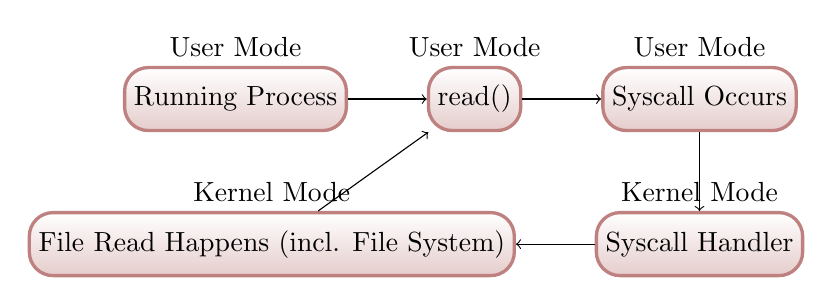
\begin{tikzpicture}[
	n_st/.style={
		rectangle,
		minimum size=8mm,
		very thick,
		draw=red!50!black!50,
		top color=white,
		bottom color=red!50!black!20,
		rounded corners=3mm,
		}]

	\node(proc)[n_st][label=User Mode]{Running Process};
	\node(readcall)[n_st, right=of proc][label=User Mode]{read()};
	\node(syscall)[n_st,right=of readcall][label=User Mode]{Syscall Occurs};
	\node(kernel)[n_st,below=of syscall][label=Kernel Mode]{Syscall Handler};
	\node(wh)[n_st, left=of kernel][label=Kernel Mode]{File Read Happens (incl. File System)};
	\path (proc) edge[->] (readcall);
	\path (readcall) edge[->] (syscall);
	\path (syscall) edge[->] (kernel);
	\path (kernel) edge[->] (wh);
	\path (wh) edge[->] (readcall);

\end{tikzpicture}
\end{document}
